 \documentclass[11pt,final]{book}
 \title{The Rook's Guide to C++}
 \date{26 November 2013}

%%%%%%%%%%%%%%%%%%%%%%%%%%%%%%%%%%%%%%%%%%%%%%%%%%%%%%%%%%%%%%%%%%%%%%%
%%                                                                    %
%% 2013-01-30:                                                        %
%%   To get the proper thumbs up:                                     %
%%     Rename the checkmark in the dingbats.sty file to, um,          %
%%  dingbatcheckmark, then use this name in the \newcommand           %
%%                                                                    %
%%%%%%%%%%%%%%%%%%%%%%%%%%%%%%%%%%%%%%%%%%%%%%%%%%%%%%%%%%%%%%%%%%%%%%%
\hyphenation{Je-re-my}
\hyphenation{Le-Blanc}
\hyphenation{Ver-gnes}
\hyphenation{Zach-a-ry}
\hyphenation{Pat-rick}
\hyphenation{Du-Harte}
\hyphenation{Ry-an}
\hyphenation{Mat-thew}
\hyphenation{Ke-vin}
\hyphenation{Wer-zing-er}
\hyphenation{Mi-chael}
\hyphenation{Ar-chie}
\hyphenation{Bo-ren-stein}
\hyphenation{Buck-ley}
\hyphenation{Ca-ma-ra}
\hyphenation{Mac-Gil-liv-ray}
\hyphenation{Li-ber}
\hyphenation{Stu-art}
\hyphenation{Ma-rone}
\hyphenation{maz-zel-lo}
\hyphenation{Mo-ra-les}
\hyphenation{Tor-res}
\hyphenation{Ne-ben-fuhr}
\hyphenation{Pat-rice}
\hyphenation{Dan-i-el}
\hyphenation{Ta-ba-ry}
\hyphenation{De-vin}
\hyphenation{Wil-li-am-i-tis}
\hyphenation{To-ny}
\hyphenation{A-dam}
\hyphenation{Wheel-er}
\hyphenation{Lo-thar}
\hyphenation{Sand-berg}
\hyphenation{Val-de-mar}
\hyphenation{Da-vies}
\hyphenation{Jo-seph}
\hyphenation{Wil-li-am}
\hyphenation{Mad-sen}
\hyphenation{Carl-ton}
\hyphenation{Do-mi-nic}
\hyphenation{Ash-ley}
\hyphenation{Da-vid}
\hyphenation{Cris-to-fo-ri}
\hyphenation{Mes-ki-men}
\hyphenation{Bran-don}
\hyphenation{Nord-garden}
\hyphenation{A-leks-an-der}
\hyphenation{Pa-da-wer}
\hyphenation{Aar-on}
\hyphenation{Mc-In-tosh}
\hyphenation{Moul-ton}
\hyphenation{niel-sen}
\hyphenation{Pon-tus}
\hyphenation{Nils-son}
\hyphenation{Mar-shall}
\hyphenation{To-ny}
\hyphenation{Wil-li-ams}
\hyphenation{Dy-lan}
\hyphenation{Wi-dis}
\hyphenation{Ste-phen}
\hyphenation{Ja-net}
\hyphenation{Maw-yer}
\hyphenation{Phi-lip}
\hyphenation{Pet-rov}
\hyphenation{Slon-ka}
\hyphenation{Til-brook}
\hyphenation{Ar-man-do}
\hyphenation{Pin-ches}
\hyphenation{Ring-man}
\hyphenation{E-man-u-el}
\hyphenation{Pe-ter-son}
\hyphenation{Rich-ard}
\hyphenation{Ko-gut}
\hyphenation{Mitch-ell}
\hyphenation{Sig-mund}
\hyphenation{Sat-tler}
\hyphenation{Le-vi}
\hyphenation{Ra-man}
\hyphenation{Ko-soy}
\hyphenation{Ja-mie}
\hyphenation{cstdlib}
\hyphenation{NetBeans}
\hyphenation{getline}
\hyphenation{setBase}

%\usepackage{arev}             % Nice heart. ($\varheart$)
%\usepackage{dingbat}          % Fists (thumbs up} (better)
%\usepackage{bbding}           % Fists (thumbs up}
%\usepackage{yfonts}           % German font(s).
%\usepackage{ulem}             % strikeout fonts.

%\newcommand{\Frak}            {\textfrak}
%\newcommand{\Frak}            {\textgoth}
%\newcommand{\Frak}            {\textswab}

%\newcommand{\F}[1]            {\Frak{#1}}

\usepackage{libertine}
\usepackage{fontspec}
\usepackage{tablefootnote}
%\usepackage{polyglossia}
%\usepackage{xunicode}
%\usepackage{xltxtra}

% Packages loaded by todonotes.  Included here so that needed options may be specified.
\usepackage{ifthen}
%\usepackage{xkeyval}
\usepackage{xcolor}
%\usepackage{tikz}
%\usepackage{calc}
\usepackage{graphicx}         % Loaded via the tikz package.
%\usepackage{todonotes}        % http://www.tex.ac.uk/tex-archive/macros/latex/contrib/todonotes/todonotes.pdf

 %\definecolor{MainFont}        {rgb}{0.000000, 0.180000, 0.180000}
 
 %\setmainfont[
 %  Color=MainFont,
 %  Opacity=0.0,
 %  Ligatures=TeX
 %  ]
 %  {Linux Biolinum}
%  {DejaVu Serif}

 %\definecolor{SansFont}        {rgb}{0.000000, 0.080000, 0.080000}
% \setsansfont[
%   Color=SansFont,
%   Opacity=0.0,
%   Ligatures=TeX
%   ]
%   {Linux Biolinum}
%  {DejaVu Sans}
 \usepackage{verbatim}
%\usepackage{wasysym}

 \usepackage{framed}
 \usepackage{layout}
\usepackage[paperwidth=6.0in, paperheight=9.0in]{geometry}
%\usepackage[paperwidth=8.5in, paperheight=11.0in]{geometry}
 \usepackage[pdfauthor={Jeremy A. Hansen, Ph.D.}, pdftitle={The Rook's Guide to C++}]{hyperref}
 \urlstyle{same}
%%%%%%%%%%%%%%%%%%%%%%%%%%%%%%%%%%%%%%%%%%%%%%%%%%%%%%%%%%%%%%%%%%%%%%%
%%                                                                   %%
%%   The listings package produces nicely-formatted source-code      %%
%% listings.                                                         %%
%%                                                                   %%
%% http://mirrors.ibiblio.org/CTAN/macros/latex/contrib/listings     %%
%%                                                                   %%
%%   We specified only the parameters necessary produce this         %%
%% document.  There are more.  Consult the package documentation     %%
%% at the above site.                                                %%
%%                                                                   %%
%% Wikibooks has a writeup, too.                                     %%
%% \href{http://en.wikibooks.org/wiki/LaTeX/Source_Code_Listings}    %%
%%     {source code listings package}                                %%
%%                                                                   %%
%%%%%%%%%%%%%%%%%%%%%%%%%%%%%%%%%%%%%%%%%%%%%%%%%%%%%%%%%%%%%%%%%%%%%%%

 \usepackage{listings}

 \usepackage{fancyhdr}
 \setlength{\headheight}{15.2pt}

 \usepackage{makeidx}
 \makeindex
 \raggedbottom
 
 \input{utils-commands.tex}


 \setcounter{tocdepth}{4}

 \begin{document}
 \maketitle
 \thispagestyle{empty}
 \newpage

 \setcounter{page}{1}
 \pagenumbering{roman}
% \pagestyle{plain}

 \thispagestyle{empty}
%% copyrightpage
\begingroup
\normalsize
\parindent 0pt
\parskip \baselineskip
\textcopyright{} 2013 Jeremy A. Hansen \\
All rights reserved.

    This work is licensed under a Creative Commons Attribution-NonCommercial-ShareAlike 3.0 Unported License, as described at 

\noindent \url{http://creativecommons.org/licenses/by-nc-sa/3.0/legalcode}

Printed in the United States of America

\vfill

\begin{center}
\begin{tabular}{ll}
First edition:  & November 2013 \\
\end{tabular}
\end{center}

\vfill

ISBN 978-1-304-66105-0

\vfill

Rook's Guide Press \\
19 Black Road \\
Berlin, VT 05602 \\
\url{http://rooksguide.org}

%%%%{\LARGE\plogo}
\vspace*{2\baselineskip}


\endgroup
%\clearpage

\newpage

 \setcounter{page}{1}


\chapter*{Preface\markboth{\MakeUppercase{Preface}}{}}

What you are reading is the first of what I hope to be many ever-improving iterations of a useful C++ textbook.
We've gone fairly quickly from whim to print on an all-volunteer basis, and as a result, there are many things that I'd add and change if I had an infinite amount of time in my schedule.
The vast majority of the contents were written in less than 36 hours by 25 students (mostly freshmen!) at Norwich University over a long weekend.
Some of it is mine, and some was added by our crack team of technical editors as we translated sleep-deprived poor grammar into sleep-deprived better grammar.

Where it goes from here is mostly up to you!
If there's a section that's missing or in need of clarification, please take a bit of time and make those changes.
If you don't want to bother yourself with the GitHub repository, send me your additions and modifications directly.

I want to first thank my family for the time I didn't spend with them on the writing weekend and throughout the summer when I was editing and typesetting. I promise I won't do this next summer!

My next thanks go out to the technical editors and typesetters, without whom you would have a much uglier book.
Thanks to Ted Rolle for building the initial \LaTeX framework and to Matt Jadud for the incredibly helpful pointers on how to manage the pile of typesetting files in a collaborative environment. I also thank Craig Robbins and Levi Schuck, who, on different sides of the planet, managed to contribute extensively to the heavy lifting of getting the book into the shape it's in now. If we ever meet, I owe you a beer or whatever you're having!

I also would like to thank all of the Kickstarter backers not only for the money which made this possible, but for reinforcing the idea that this is a worthwhile contribution to the community. Peter Stephenson and Andrew Pedley also contributed food directly over the textbook writing hackathon weekend, and without them we'd never have gotten our saturated fat quota! (Note to future project leaders: there's nothing that gets a bunch of college students who are generally lukewarm about programming to write a textbook like free food. It didn't even matter what the food was. Really.)

Thanks to Matt Russo for shooting the video and organizing the media and social networking efforts with the Kickstarter project through the writing weekend.

Special thanks to Allyson LeFebvre\footnote{That's ``la-fave'', everyone} for the textbook photography, several diagrams, and the extensive search through the semi-final textbook that turned up a bunch of mistakes that I missed.

And my last (and not at all least) thanks go out to all the students who showed up in person or digitally. And without getting too grandiose, you remind us all that we can make the world better by showing up. Keep showing up!

~ \linebreak

\noindent \textbf{Jeremy}

\noindent \texttt{jeremyhansen@acm.org}

\noindent 26 November 2013

~ \linebreak

\pagebreak 

 \tableofcontents

%%%%%%%%%%%%%%%%%%%%%%%%%%%%%%%%%%%%%%%%%%%%%%%%%%%%%%%%%%%%%%%%%%%%%%%
%%                                                                   %%
%%   Here are the listing package's parameters used in the creation  %%
%% of this book.                                                     %%
%%                                                                   %%
%%%%%%%%%%%%%%%%%%%%%%%%%%%%%%%%%%%%%%%%%%%%%%%%%%%%%%%%%%%%%%%%%%%%%%%
\input{utils-listings.tex}


 %\Comment{ % Frontmatter.

\chapter*{License\markboth{\MakeUppercase{License}}{}}


\vspace{1in}

\includegraphics[width=.25\textwidth]{graphics/cc.large.png} \
\includegraphics[width=.25\textwidth]{graphics/by.large.png} \
\includegraphics[width=.25\textwidth]{graphics/nc.large.png} \
\includegraphics[width=.25\textwidth]{graphics/sa.large.png}

\vspace{1in}



\noindent This work by Jeremy A. Hansen (jeremyhansen@acm.org) is licensed under a Creative Commons Attribution-NonCommercial-ShareAlike 3.0 Unported License, as described at \newline

\noindent \footnotesize \url{http://creativecommons.org/licenses/by-nc-sa/3.0/legalcode}





% \\A \href{http://creativecommons.org/licenses/by-nc/3.0/}


\chapter*{Dramatis Person\ae\markboth{\MakeUppercase{Dramatis Person\ae}}{}}

 \begin{description}

 \item[Managing Editor:] ~
 
 Jeremy A. Hansen, PhD, CISSP

 \item[Technical Editing \& Typesetting:] ~
 
 Jeremy A. Hansen
 
 Matt Jadud, PhD
 
 Craig D. Robbins
 
 Theodore M. Rolle, Jr.
 
 Levi Schuck

 \item[Media \& Outreach:] ~
 
 Matthew E. Russo

 \item[Cover Art \& Graphic Design:] ~
 
 Allyson E. LeFebvre

 \item[Content Authors:]\label{ContentAuthors} ~
 
Tyler Atkinson,
Troy M. Dundas,
Connor J. Fortune,
Jeremy A. Hansen,
Scott T. Heimann,
Benjamin J. Jones,
Michelle Kellerman,
Michael E. Kirl,
Zachary LeBlanc,
Allyson E. LeFebvre,
Gerard O. McEleney,
Phung P. Pham,
Megan Rioux,
Alex Robinson,
Kyle R. Robinson-O'Brien,
Jesse A. Rodimon,
Matthew E. Russo,
Yosary Silvestre,
Dale R. Stevens,
Ryan S. Sutherland,
James M. Verderico,
Christian J. Vergnes,
Rebecca Weaver,
Richard Z. Wells, and
Branden M. Wilson.

 \item[Funding \& Support:] ~
 
Peter Stephenson, PhD, VSM, CISSP, CISM, FICAF, LPI at the Norwich University Center for Advanced Computing \& Digital Forensics

Andrew Pedley at Depot Square Pizza
 \end{description}

\noindent \textbf{Kickstarter contributors:}   

\noindent \input{kickstarters.tex}

% } % End Frontmatter Comment.

% \LevelA{Section 1}
   %\LevelB{Chapters:}
      \LevelC{History}
 \setcounter{page}{1}
 \pagenumbering{arabic}
 %\pagestyle{fancy}
			\label{chap_history}
      % This work by Jeremy A. Hansen is licensed under a Creative Commons 
% Attribution-NonCommercial-ShareAlike 3.0 Unported License, 
% as described at http://creativecommons.org/licenses/by-nc-sa/3.0/legalcode

Developed by Bjarne Stroustrup, C++ has become one of the most popular programming languages in the world. 
Originally, it was designed as an improvement upon the C language, which was developed by Bell Labs. 
Developed in the early 1970s, C's name is derived from the B programming language, which in turn was derived from the BCPL language. 
C gained a large following, in part due to its use in the development of the UNIX operating system. 
Due to both its popularity and the number of versions on the market, an American National Standards Institute (ANSI) committee was formed in 1982 to create a standard for the C language, which was adopted in 1989.

Stroustrup began with the idea that object oriented programming would be an important addition to C, and created C with Classes.
In 1983, Stroustrup's contributions officially became known as C++, its name stemming from C and adding the Code{++} (increment) operator. 
It wasn't until 1998 that the international standard for C++ was established.

Since then, most changes have been minor. 
In 2005, a report was released by the ISO on features that were intended to be included in the next version of C++. 
The early versions of this became known as C++0x, until 2011, when the C++11 standard was released by the ISO.

In this book, we'll favor older techniques, pre-C++11. 
When C++11 features are discussed, they will be pointed out as such. 
While not all of the new features are discussed, we will be trying our best to explain them as we go.

%      \LevelC{Types of languages}
%      \input{chap_types.tex}
%      \LevelC{How Computers Use Memory}
%      \input{chap_memory.tex}
%      \LevelC{Sample Program}
%			\label{chap_sampleprogram}
%      \input{chap_sampleprogram.tex}
      \LevelC{Your First Program}
			\label{chap_firstprogram}
      % This chapter by Robert J. Garner is licensed under a Creative Commons 
% Attribution-NonCommercial-ShareAlike 3.0 Unported License, 
% as described at http://creativecommons.org/licenses/by-nc-sa/3.0/legalcode

To begin learning programming students are often asked to create a simple "hello world" program. In this chapter you will learn the following:


\begin{itemize}
\item Install software needed to write code.
\item Start a new solution/project.
\item Write a simple program (Hello World!).
\end{itemize}

\LevelD{Basic Process}
The basic process for creating a program consists of the following:
\begin{enumerate}
\item Write a program using a text editor.
\item Compile the program using a program called a compiler.
\item Link the program using a program called a linker.
\end{enumerate}
While it is possible to accomplish all of these steps manually, there are programs today called Integrated Development Environments (IDEs) that will handle each of these operations for you and provide an integrated environment to write your code and build it. 

\LevelD{Software Required}
The IDE we will use for this example is a program called Microsoft Visual Studio{TM}. 
You can download a free version from \url{www.visualstudio.com/en-us/products/visual-studio-express-vs.aspx}. 
Alternatively if you are a student you can sign up for a Microsoft DreamSpark account at \url{www.dreamspark.com/}.
Microsoft's DreamSpark{TM} program provides students free access to Microsoft{TM} software. To install the software follow the instructions on the website from which you download it.
 

\LevelD{Working With the IDE}
Once your IDE is installed you should become familiar with the following basic functions:

\begin{itemize}
\item Basic layout of the IDE
\item Opening Windows
\item Re sizing and Moving Windows
\Item Arranging you workspace efficiently
\end{itemize}
\LevelE{Basic layout of the IDE}

Figure 2.1 shows what the Visual Studio interface looks like. If you are familiar with office applications you will recognize several of the menu items such as File, Edit and View. These menus will do much of the same types of functions that they do in other applications. Initially an IDE can be overwhelming to a new programmer because there are many functions and often there are multiple ways of doing the same thing.

\begin{figure}[tb]
  \centering
  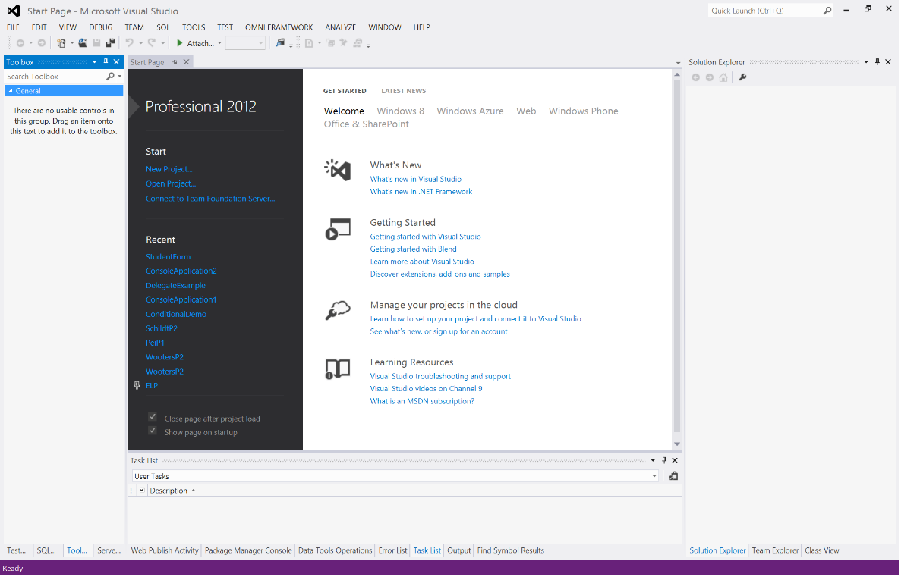
\includegraphics[width=\textwidth]{diagrams/visual_studio_start_page.pdf}
  \caption{Visual Studio Start Page} \label{fig-if-flowchart}
\end{figure}
\LevelD{Creating A New Solution}





% \LevelA{Section 2}
   %\LevelB{Chapters:}
     \LevelC{Variables}
			\label{chap_variables}
      \input{chap_variables.tex}
     \LevelC{Literals and Constants}
			\label{chap_constants}
      \input{chap_constants.tex}
     \LevelC{Assignments}
			\label{chap_assignments}
      \input{chap_assignments.tex}
     \LevelC{Output}
			\label{chap_output}
      \input{chap_output.tex}
     \LevelC{Input}
			\label{chap_input}
      \input{chap_input.tex}
     \LevelC{Arithmetic}
			\label{chap_arithmetic}
      \input{chap_arithmetic.tex}
     \LevelC{Comments}
			\label{chap_comments}
      \input{chap_comments.tex}
     \LevelC{Data Types and Conversion}
			\label{chap_datatypes}
      \input{chap_datatypes.tex}

% \LevelA{Section 3}
%   \LevelB{Chapters:}
     \LevelC{Conditionals}
			\label{chap_conditionals}
      \input{chap_conditionals.tex}
     \LevelC{Strings}
			\label{chap_strings}
      \input{chap_strings.tex}
     \LevelC{Loops}
      \label{chap_loops}
      \input{chap_loops.tex}
     \LevelC{Arrays}
			\label{chap_arrays}
      \input{chap_arrays.tex}
     \LevelC{Blocks, Functions, and Scope}
			\label{chap_functions}
      \input{chap_functions.tex}
     \LevelC{Problem Solving \& Troubleshooting}
			\label{chap_problems}
      \input{chap_problems.tex}
%     \LevelC{Testing}
%			\label{chap_testing}
%      \input{chap_testing.tex}

% \LevelA{Section 4}
%   \LevelB{Chapters}
     \LevelC{The Preprocessor}
			\label{chap_preproc}
      \input{chap_preproc.tex}
     \LevelC{Advanced Arithmetic}
			\label{chap_advancedarith}
      \input{chap_advancedarith.tex}
     \LevelC{File I/O}
			\label{chap_file_io}
      \input{chap_file_io.tex}
     \LevelC{Pointers}
			\label{chap_pointers}
      \input{chap_pointers.tex}
     \LevelC{Dynamic Data}
			\label{chap_dynamic}
      \input{chap_dynamic.tex}

 \Comment{ % LevelX comment.

 \LevelA{}
   \LevelB{}
     \LevelC{}
     \LevelC{}
     \LevelC{}
     \LevelC{}
     \LevelC{}
     \LevelC{}
     \LevelC{}
     \LevelC{}
 } % End LevelX comment.

% \LevelA{Section 5}
%   \LevelB{Chapters}
%     \LevelC{User-defined types}
%      \input{chap_userdefined.tex}
     \LevelC{Classes and Abstraction}
			\label{chap_classes}
      \input{chap_classes.tex}
%     \LevelC{Exceptions}
%      \input{chap_exceptions.tex}
     \LevelC{Separate Compilation}
			\label{chap_separate}
      \input{chap_separate.tex}
     \LevelC{The C++ Standard Library}
			\label{chap_stl}
      \input{chap_stl.tex}

 %\missingfigure{Pictures and figures and tables are a nice touch.}

 %\listoftodos

 %\lstlistoflistings

 \printindex

 \end{document}
